\section{Result and Discussion}
\label{sec:resultdiscussion}

\subsection{Accuracy Testing Scenario}
\label{sec:skenariopengujian}

The accuracy test is done by placing the ball in the middle of the field with the actual coordinates of {400, 600}. Then place the robot at a distance of 120 cm, 200 cm, and 285 cm from the ball and rotate the robot in place. Every 30 degrees, the robot will record the ball position on the field resulting from the calibration implementation. Then the results will be calculated the \emph{Euclidean Distance} between the actual ball position and the ball position resulting from the calibration. The following is the testing scenario that was carried out:

\begin{figure}[H]
  \centering
  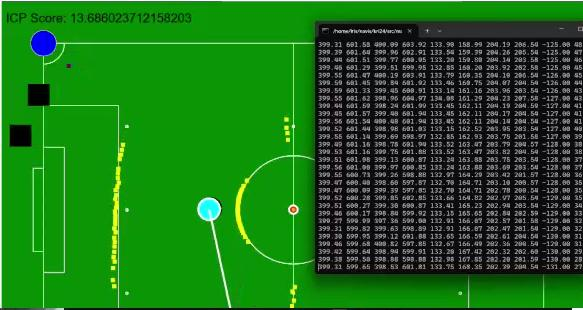
\includegraphics[width=8cm]{gambar/saat_putar_bola_2.jpeg}
  \caption{Testing Scenario.}
  \label{fig:skenariopengujian}
\end{figure}

\subsection{Accuracy Testing Evaluation}
\label{sec:analisispengujian3}

While the test is running, the robot will rotate in its position to detect the ball on the field. The robot will rotate 30 degrees each time. The robot will rotate 12 times so that the robot can see the ball from all directions. After the robot has finished rotating, the robot will stop and the data will be recorded. The data obtained is the ball position on the field. The data is then compared with the actual ball position on the field. There are three tests that have been carried out, namely at a distance of 120 cm, 200 cm, and 285 cm. The following is the evaluation of the test results. The following data is obtained from the test results:

% Example of making a table

\begin{table}[H]
  \caption{Ball Position Test Results on the Field with a Distance of 120 cm using Machine Learning.}
  \begin{center}
    \begin{tabular}{|c|c|c|c|}
      \hline
    \rowcolor[HTML]{C0C0C0}
  \textbf{Angle to Ball} & \textbf{Ball Pos X} & \textbf{Ball Pos Y} & \textbf{Distance Error} \\
  \hline
  0 deg            & 407.74 cm                & 596.67 cm    & 8.42 cm        \\
  30 deg           & 409.41 cm                & 600.3 cm     & 9.41 cm        \\
  60 deg           & 409.65 cm                & 600.54 cm    & 9.66 cm         \\
  90 deg           & 407.52 cm                & 598.2 cm      & 7.73 cm      \\
  120 deg           & 407.18 cm                & 600.07 cm    & 7.18 cm        \\
  150 deg           & 409.98 cm                & 598.35 cm     & 10.11 cm       \\
  180 deg           & 410.66 cm                & 593.41 cm     & 12.53 cm       \\
  210 deg           & 410.84 cm                & 590.28 cm    & 14.55 cm        \\
  240 deg           & 410.01 cm                & 590.8 cm     & 13.59 cm      \\
  270 deg           & 409.9 cm                & 594.28 cm     & 11.43 cm      \\
  300 deg           & 408.91 cm                & 590.14 cm    & 13.28 cm       \\
  330 deg           & 408.8 cm                & 591.57 cm    & 12.18 cm       \\
  \hline
\end{tabular}
\end{center}
\end{table}


From that data, we can calculate the average error distance. The following is the calculation of the average error distance:

\begin{equation}
  \text{Avg error} = \frac{\sum \text{Distance Error}}{12} = \frac{123.64}{12} = 10.3 \text{ cm}
\end{equation}

So that we can conclude the Accuracy Error is 10.3 cm. 


\subsection{Precision Testing Testing Scenario}
\label{sec:skenariopengujian2}

The Precision Testing test is comparing the Machine Learning Calibration results with the Polynomial Regression Calibration that still uses the \emph{polynomial regression} algorithm. The test is done in the same way as the previous accuracy test. However, the Camera Calibraion process uses the \emph{polynomial regression} algorithm.

\subsection{Precision Testing Testing Evaluation}
\label{sec:32}

The test is done by comparing the data obtained from the Machine Learning Calibration with the data obtained from the Polynomial Regression Calibration. The following is the data obtained from the test results: 

\begin{table}[H]
  \caption{Ball Position Test Results on the Field with a Distance of 120 cm using Machine Learning.}
  \begin{center}
    \begin{tabular}{|c|c|c|}
      \hline
    \rowcolor[HTML]{C0C0C0}
  \textbf{Robot Angle to Ball} & \textbf{Ball Position X} & \textbf{Ball Position Y} \\
  \hline

  0 deg            & 407.74 cm                & 596.67 cm            \\
  30 deg           & 409.41 cm                & 600.3 cm            \\
  60 deg           & 409.65 cm                & 600.54 cm            \\
  90 deg           & 407.52 cm                & 598.2 cm           \\
  120 deg           & 407.18 cm                & 600.07 cm           \\
  150 deg           & 409.98 cm                & 598.35 cm           \\
  180 deg           & 410.66 cm                & 593.41 cm           \\
  210 deg           & 410.84 cm                & 590.28 cm           \\
  240 deg           & 410.01 cm                & 590.8 cm           \\
  270 deg           & 409.9 cm                & 594.28 cm           \\
  300 deg           & 408.91 cm                & 590.14 cm           \\
  330 deg           & 408.8 cm                & 591.57 cm           \\
  \hline
\end{tabular}
\end{center}
\end{table}

\begin{table}[H]

\caption{Ball Position Test Results on the Field with a Distance of 120 cm using the Polynomial Regression.}
\begin{center}

\begin{tabular}{|c|c|c|}
  \hline
  \rowcolor[HTML]{C0C0C0}
  \textbf{Robot Angle to Ball} & \textbf{Ball Position X} & \textbf{Ball Position Y} \\
  \hline
  0 deg            & 370.18 cm                & 576.31 cm            \\
  30 deg           & 376.24 cm                & 585.42 cm            \\
  60 deg           & 383.91 cm                & 597.98 cm            \\
  90 deg           & 392.99 cm                & 605.67 cm           \\
  120 deg           & 390.23 cm                & 610.94 cm           \\
  150 deg           & 400.49 cm                & 598.89 cm           \\
  180 deg           & 385.97 cm                & 582.89 cm           \\
  210 deg           & 398.61 cm                & 577.15 cm           \\
  240 deg           & 390.76 cm                & 585.02 cm           \\
  270 deg           & 386.32 cm                & 588.91 cm           \\
  300 deg           & 378.69 cm                & 585.55 cm           \\
  330 deg           & 370.32 cm                & 579.11 cm           \\
  \hline
\end{tabular}
\end{center}
\end{table}

From the data, it can be seen that the standard deviation in the ball position data on the field with a distance of 120 cm using the Polynomial Regression Calibration is 10.01 cm and 11.32 cm for the ball position x and y. Meanwhile, in the Machine Learning Calibration, the standard deviation is 1.26 cm and 4.11 cm for the ball position x and y. It can be seen that the Machine Learning Calibration is better than the Polynomial Regression Calibration. This happens because the camera is not installed correctly on the robot, causing the Polynomial Regression Calibration results to be inaccurate. The inaccuracy occurs because the Polynomial Regression Calibration only uses one direction as a reference for the polynomial regression model. Whereas, in reality, the model formula for each camera direction will always be different.

% \subsection{Third Accuracy Testing}
% \label{sec:skenariopengujian3}

% The third accuracy test is placing robot somewhere on the field and then the robot will see lines around the robot. The robot will detect each pixel of line and then the robot will calculate the distance between the robot and the line. So the robot can visualize the line on the field. The test is done by taking data from the omnivision camera that has been installed on the robot and then processing the data using the \emph{Lookup Table} that has been created before so that the line coordinates on the field are obtained. The following is the testing scenario that was carried out: 

% \begin{figure}[H]
%   \centering
%   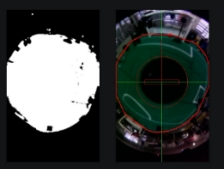
\includegraphics[width=7cm]{gambar/cam_raw1.jpg}
%   \caption{Raw frame.}
%   \label{fig:skenariopengujian31}
% \end{figure}

% The left picture is the field binary image that calculated to get the line binary image. 

% \begin{figure}[H]
%   \centering
%   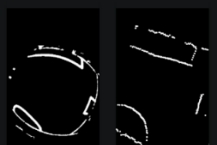
\includegraphics[width=7cm]{gambar/cam_raw2.jpg}
%   \caption{Calculated frame.}
%   \label{fig:skenariopengujian32}
% \end{figure}

% The left picture is the line binary image that calculated to get the line coordinates on frame. Extracting the line coordinates on the frame is done by scanning from the center of frame to the edge of frame.  

% \begin{algorithm}[H]
%   \caption{Process Lines on Frame}\label{alg:process_lines}
%   \begin{algorithmic}[1]
%   \Procedure{ProcessLinesOnFrame}{}
%       \State \text{Initialize lines\_on\_frame as an empty vector}
%       \For{\text{angle from 0 to 360 with step size 2.5}}
%           \State \text{Initialize dist to 0}
%           \For{\text{index from 0 to 320}}
%               \State $x \gets \text{dist} \times \cos(\text{angle}) + \text{center\_cam\_x}$
%               \State $y \gets \text{center\_cam\_y} - \text{dist} \times \sin(\text{angle})$
%               \If{\text{frame[y][x] == 255}}
%                   \State \text{Push (x, y) to lines\_on\_frame}
%               \EndIf
%               \State $dist \gets \text{dist} + 1$
%           \EndFor
%       \EndFor
%   \EndProcedure
%   \end{algorithmic}
% \end{algorithm}

% % Dummy
% After getting the line coordinates on the frame, the robot will calculate the world coordinates of the line. The formula used to calculate the line's position on the field is as follows:

% \begin{equation}
%   \begin{aligned}
%     dx &= x\_line\_cam - x\_center\_cam \\
%     dy &= y\_center\_cam - y\_line\_cam \\
%     r\_line\_cam &= \sqrt{dx^2 + dy^2} \\
%     \theta\_line\_cam &= \arctan(\frac{dy}{dx}) \\
%     index &= \theta\_line\_cam \times r\_max + r\_line\_cam \\ 
%     r\_line\_fld &= r\_lookup[index] \\
%     \theta\_line\_fld &= \theta\_line\_cam + robot\_\theta - 90 \\
%     x\_line &= robot\_x + r\_line\_fld \times \cos(\theta\_line\_fld) \\
%     y\_line &= robot\_y + r\_line\_fld \times \sin(\theta\_line\_fld) \\
%   \end{aligned}
% \end{equation}

% After the robot has finished calculating the line's position on the field, the robot will visualize the line on the field. The visualization can be seen on right picture of figure \ref{fig:skenariopengujian32}.


\subsection{Computational Speed Testing Scenario}
\label{sec:30}

The test is done by comparing whether the Machine Learning Calibration system is faster than using the Polynomial Regression Calibration system. The test is done by recording the time after calibration and subtracting it from the time before calibration. So that an estimate of the time it takes for the system to perform the calculation process for calibration can be obtained. The following formula is used to calculate the delay time:

\begin{equation}
  \begin{aligned}
    delay\_time &= time1 - time0 \\ 
  \end{aligned}
\end{equation}

Where $time1$ is the time after calibration and $time0$ is the time before calibration.

\subsection{Computational Speed Testing Evaluation}
\label{sec:31}

From the tests that have been carried out, there are 10 iterations that have been done. The following is the data obtained from the test results:

\begin{table}[htpb]
  \caption{Difference in Computational Speed Test Results}
\begin{center}

\begin{tabular}{|c|c|c|}
  \hline
  \rowcolor[HTML]{C0C0C0}
  \textbf{Iteration to-} & \textbf{New Calibration Time} & \textbf{Old Calibration Time} \\
  \hline
  0            & 119 ns                & 176 ns            \\
  1           & 76 ns                & 86 ns            \\
  2           & 25 ns                & 107 ns            \\
  3           & 31 ns                & 90 ns           \\
  4           & 32 ns                & 88 ns           \\
  5           & 36 ns                & 87 ns           \\
  6           & 37 ns                & 88 ns           \\
  7           & 34 ns                & 93 ns           \\
  8           & 37 ns                & 89 ns           \\
  9           & 35 ns                & 90 ns           \\
  \hline
\end{tabular}
\end{center}
\end{table}

With New Calibration Time stand for the Machine Learning Calibration system and Old Calibration Time stand for the Polynomial Regression Calibration system.

From the graph, it can be seen that the Machine Learning Calibration system is 53.2 ns faster than the Polynomial Regression Calibration system. With an average of 46.2 ns for the Machine Learning Calibration and 99.4 ns for the Polynomial Regression Calibration. This is because the Machine Learning Calibration system only uses a \emph{Lookup Table} containing camera calibration data. Whereas the Polynomial Regression Calibration system uses the polynomial regression algorithm which takes longer.


